\chapter{attract mode admin}
\label{sec:attract_mode}
\lhead[tempest]{}
\lstset{style=6502Style}

There is naturally a bit of administrative overhead associated with operating
a game in 'attract mode'. In case you may be wondering, 'attract mode' is when a game cabinet
sits unattended and is attempting to attract customers. The manufacturer can display a colourful title
screen and high score tables, maybe play a tune. But often the most effective way of getting
people to play your game is to show the game being played. This allows the uninitiated to get a sense
of what they're missing out on and also gives them an idea of how to proceed when they
enter their first coin.
Providing this kind of demonstration gameplay means devising some rudimentary intelligence in the game logic that will
mimic the activity of a fairly competent paying customer. Fortunately, in \textit{Tempest}
there are only
two things that a player actually does: move and shoot. This means that our task of 
emulating a player negotiating a level in \textit{Tempest} is simpler
than it might at first appear. We can split it out into two separate concerns, and if we solve 
each one we will have an artificial player that can help bring in some business.

When we get our 'attract mode' up and running we have a small bit of setup to
perform first. The demonstration player is only given one life, and the level they
will play is chosen at random from the first eight.
\begin{lstlisting}
        BIT QSTATUS   ; CHECK FOR ATTRACT MODE..
        IFPL          ; IF IT IS ENABLED THEN..
        LDY I,1       ; LOAD 1 INTO Y REGISTER.
        STY LIVES1    ; AND STORE THAT AS AVAILABLE LIVES.
        LDA RANDOM    ; STORE A RANDOM NUMBER IN ACCUMULATOR.
        AND I,7       ; CLAMP IT TO BETWEEN 0 AND 7.
        ENDIF
        STA X,WAVEN1  ; USE THE RANDOM NUM TO SELECT LEVEL.
        STA CURWAV    ; STORE IT AS THE CURRENT LEVEL TOO.
\end{lstlisting}

With this environment for our player established we can first figure out how to make
him move.
\section*{movement admin}
This one is surprisingly easy. At any given moment we just have to decide whether
the cursor (representing the player) is going to move left or right. The only thing
that should ever affect this decision is whether the movement moves us nearer the same
line as the furthest advanced enemy that we can shoot at. 

\begin{lstlisting}
        .SBTTL PLAY - MOVE CURSOR (MAINLINE)
        LDX I,0
        LDA QSTATUS
        IFPL                    ;ATTRACT?
        JSR AUTOCU              ;YES, AUTO MOVEMENT
\end{lstlisting}

\begin{minipage}[c]{0.48\linewidth}
\begin{figure}[H]
    \centering
    \begin{adjustbox}{width=6cm,center}
      \includegraphics[width=3cm]{src/attractmode/movement_example1_before.png}%
    \end{adjustbox}
\end{figure}
\end{minipage}
\begin{minipage}[c]{0.06\linewidth}
\begin{figure}[H]
    \centering
    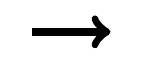
\begin{tikzpicture}[baseline={(current bounding box.south)}]
      \draw[->,line width=3pt] (0,0) to (1,0);
    \end{tikzpicture}
\end{figure}
\end{minipage}
\begin{minipage}[c]{0.48\linewidth}
\begin{figure}[H]
    \centering
    \begin{adjustbox}{width=6cm,center}
      \includegraphics[width=3cm]{src/attractmode/movement_example1_after.png}%
    \end{adjustbox}
\end{figure}
\end{minipage}


Routine for moving the cursor automatically.
\begin{lstlisting}
  .SBTTL  PLAY-AUTO MOVE OF CURSOR
AUTOCU: 
  LDA I,-1        ; STORE -1 IN THE ACCUMULATOR.
  STA TEMP0       ; USE IT TO INITIALISE TEMP0.
  STA TEMP1       ; USE IT TO INITIALISE TEMP1.

  ; GET THE INDEX OF THE INVADER THAT IS FURTHEST ADVANCED
  ; ALONG THE WEB.
  LDX WINVMX      ; GET THE NUMBER OF INVADERS.
  BEGIN           ; LOOP FOR ALL INVADERS
    LDA X,INVAY   ; GET CURRENT INVADER'S DEPTH POSITION. 
    IFNE          ; IF IT HAS ONE THEN..
      CMP TEMP0   ; IS IT THE HIGHEST SO FAR?
      IFCC        ; IF IT IS THEN..
      STA TEMP0   ; STORE THE NEW HIGHEST POSITION.
      STX TEMP1   ; STORE THE INDEX OF HIGHEST INVADER.
      ENDIF
    ENDIF
    DEX           ; GO THE NEXT INVADER.
  MIEND           ; LOOP UNTIL WE'VE CHECKED THEM ALL.

  ; FIGURE OUT IF MOVING LEFT OR RIGHT GETS US NEARER TO THE
  ; FURTHEST ADVANCED INVADER.
  LDX TEMP1      ; STORE INDEX TO FURTHEST ADVANCED INVADER IN X.
  IFPL           ; IF WE FOUND ONE THEN..
    LDA X,INVAL1 ; GET THE LINE THE INVADER IS ON.
    LDY CURSL1   ; GET THE LINE THE PLAYER IS ON.
    JSR POLDEL   ; CALCULATE HOW FAR AWAY ONE IS FROM THE OTHER. 
    TAY          ; STORE THE RESULT IN Y REGISTER.
    IFNE         ; IF PLAYER IS NOT ALREADY ON SAME LINE AS ENEMY..
      IFPL       ; THEN IF RESULT FROM POLDEL IS POSITIVE..
      LDA I,-9   ; MOVE LEFT..
      ELSE       ; OTHERWISE..
      LDA I,9    ; MOVE RIGHT.
      ENDIF
    ENDIF
  ENDIF
  RTS
\end{lstlisting}

\section*{shooting admin}
Routine for firing a charge automatically.
\begin{lstlisting}
        .SBTTL PLAY - FIRE PLAYER CHARGE
FIREPC:
        LDA CURSL2
        IFPL                    ;PLAYER ALIVE
        LDA QSTATUS
        IFPL                    ;ATTRACT?
        LDA CURMOD              ;YES. AUTO FIRE
        STA TEMP0
        LDX I,NICHARG+NINVAD-1
        BEGIN                   ;LOOP FOR EACH INVADER & SHOT UNTIL EXHAUSTED OR CLOSE 1 IS FOUND
        LDA X,CHARY+NPCHAR
        IFNE                    ;ACTIVE?
        LDA X,CHARL1+NPCHAR     ;YES CALUCLATE ABSOLUTE VALUE OF LINE DELTA
        SEC                     ;
        SBC CURSL1
        IFMI
        EOR I,0FF
        CLC
        ADC I,1
        ENDIF
        CMP I,2
        IFCC                    ;TOO CLOSE?
        INC TEMP0               ;YES. FIRE
        ENDIF
        ENDIF
        DEX
        MIEND
        LDA TEMP0
        ELSE
        LDA SWSTAT
        AND I,MFIRE
        ENDIF
        IFNE                    ;FIRE CHARGE?
        LDX I,NPCHARG-1         ;YES
        BEGIN                   ;LOOP UNTIL VACANCY IS FOUND
        LDA X,CHARY
        IFEQ                    ;VACANCY?
                                ;YES FIRE CHARGE
        INC CHACOU
        LDA CURSY               ;START AT CURSOR
        STA X,CHARY
        LDA CURSL1
        STA X,CHARL1            ;STARTS AT SAME LINE AS CURSOR
        LDA CURSL2
        STA X,CHARL2
        LDA I,0                 ;0 COLLISION COUNTER
        STA X,CHARCO
        JSR SLAUNC              ;LAUNCH SOUND
        LDA CURSY
        JSR COLCHK              ;CHECK FOR COLLISION
        LDX I,0                 ;EXIT LOOP
        ENDIF
        DEX
        MIEND
        ENDIF
        ENDIF
        RTS
\end{lstlisting}

Put the game into attract mode when displaying the high score table.
\begin{lstlisting}
DLADR:  LDA QSTATUS
        AND I,^C<MATRACT!MGTMOD>
                        ;PUT INTO ATTRACT
        STA QSTATUS             ;REQUEST DISPLAY OF LADDER
        LDA I,0                 ;
        STA NUMPLA              ;RETURN TO PLAYER
        LDA I,CLOGO
        STA QNXTSTA             ;REQUEST NEW GAME AFTER
        LDA I,CPAUSE            ;A LONG DELAY
        STA QSTATE
        LDA I,0A0
        STA QTMPAUS
        LDA I,1                 ;DOUBLE TIME
        STA PSCALE
        LDA I,CDHITB
        STA QDSTATE
        RTS
\end{lstlisting}
